\documentclass[12pt,oneside,a4paper]{book} % Document Style with 12 point spacing, onesided sheets of a4. This is a book type of document.

%Packages
\usepackage{ecproject}
\usepackage{graphicx}
\usepackage{tikz}
\usetikzlibrary{calc}
\usepackage[a4paper, margin=1in]{geometry}
\usepackage{float}
\usepackage{qrcode}
%%%Page related
\usepackage{fancyhdr} % for header & footer
\usepackage[hidelinks]{hyperref}
\usepackage[toc, acronym, nonumberlist]{glossaries} %For Glossaries - to be loaded only after hyperref package
%\ifIndentPara
\usepackage{indentfirst}
%\fi
\usepackage{setspace}
%%%Table Related
%\usepackage{booktabs}
%\usepackage{makecell}
%\usepackage{multirow}
%\usepackage{multicol}
 % Contains the supporting packages needed to compile the latex document

\title{Development of MCM-MIMO Processing for Urban Cellular Link
} %The title of the project
\MinorProject %Tells Latex to use the Minor project style defined in ecproject.sty file

%%%Student Details%%%
\stuNameA{Nagendra Kumar Jamadagni}
\stuUSNA{1RV17EC083}
\stuNameB{Nischith T.R}
\stuUSNB{1RV17EC093}

%Guide Details%%%%
\guideNameA{Dr. S Ravi Shankar}
\guideDesignationA{Professor}
\guideDeptA{Dept. of ECE}
\guideOrgA{RV College of Engineering}

%Panel Members Details%%%

\panelMemberA{Dr. S Ravi Shankar}
\panelMemberDesigA{Professor}
\panelMemberB{Dr. Shushrutha K.S.}
\panelMemberDesigB{Associate Professor}

\Department[ECE]{Electronics and Communication Engineering}

\HOD{Dr. K S Geetha}
\Principal{Dr. K. N. Subramanya}

\academicYear{2020-2021}
\QRurl{https://drive.google.com/drive/u/1/folders/1n9KovYaUDG43-PdKLFIAwKlocxBlZOo5} %Add QR Code URL to the brackets. Only if we are generating.
\DeclarePairedDelimiter{\nint}\lfloor\rceil
\DeclarePairedDelimiter\abs{\lvert}{\rvert}
\DeclarePairedDelimiter\norm{\lVert}{\rVert}
\DeclarePairedDelimiter\ceil{\lceil}{\rceil}
\DeclarePairedDelimiter\floor{\lfloor}{\rfloor}


\DraftCopy

%Add glossaries from glossaries.tex file
\newglossary[sym]{symbolList}{sym1}{sym2}{List of Symbols}
\makeglossaries
\loadglsentries{./Supporting Files/Glossaries}
\renewcommand{\glspostdescription}{}% To remove dot at the end
\renewcommand{\listalgorithmname}{LIST OF ALGORITHMS}   


%To add references in IEEE style
\usepackage[backend=biber, style=ieee]{biblatex}
\addbibresource{./Supporting Files/References.bib}


%To add RV Logo as a watermark
\usepackage{eso-pic}
\AddToShipoutPictureFG{
          \begin{tikzpicture}[remember picture, overlay]
              \node[opacity=0.5, inner sep=0, scale=0.5] at (current page.center)
                  {\includegraphics{Common Figures/RV_logoVecw}};
          \end{tikzpicture}
}



% Start of the report/document%

\begin{document}
\maketitle %Add the title page

\newpage
\begin{spacing}{1.5}
%%ecproject package is created by P Narashimaraja, Assistant Professor, ECE, RVCE
%Border
\begin{tikzpicture}[remember picture, overlay]
  \draw[line width = 4pt] ($(current page.north west) + (0.75in,-0.75in)$) rectangle ($(current page.south east) + (-0.75in,0.75in)$);
\end{tikzpicture}
\thispagestyle{empty}
\vspace{-1cm}
\begin{center}
\Large\textbf{RV College of Engineering\textsuperscript{\small\textregistered}, Bengaluru} \par
\large{(\textit{Autonomous institution affiliated to VTU, Belagavi})} \par
\large\textbf{Department of \printDepartmentLF}\\
.\hspace{2cm}\\

\includegraphics[width=4cm]{Common Figures/RV_logoVec}\par
\Large\textbf{\underline{CERTIFICATE}} \par
\end{center}
%\begin{minipage}[b]{\linewidth}
%\large
\begin{spacing}{1.5}
\noindent Certified that the \ifMinor{minor\;}\else{ major\;}\fi project work titled \textbf{\textit{\printTitle}} is carried out by
\ifPG{%
\textbf{\printStuNameA} (\textbf{\printStuUSNA}) who is  bonafide student 
}
\else{ 
\ifStuNameCUsed{%
\textbf{\printStuNameA } (\textbf{\printStuUSNA}), \textbf{\printStuNameB } (\textbf{\printStuUSNB}) and \textbf{\printStuNameC } (\textbf{\printStuUSNC})  who are bonafide students 
}\else{%
\ifStuNameBUsed{%
\textbf{\printStuNameA} (\textbf{\printStuUSNA}) and \textbf{\printStuNameB} (\textbf{\printStuUSNB})  who are bonafide students 
}\else{%
\textbf{\printStuNameA} (\textbf{\printStuUSNA}) who is  bonafide student 
}
\fi
}\fi
}\fi
of RV College of Engineering, Bengaluru, in partial fulfillment of the requirements for the degree of  \ifPG \textbf{\printMastersInLF} in \textbf{\printMastersPrgName} \else\textbf{Bachelor of Engineering} in \textbf{\printDepartmentLF} \fi of the Visvesvaraya Technological University, Belagavi during the year \printAcadYear. It is certified that all corrections/suggestions indicated for the Internal Assessment have been incorporated in the \ifMinor{minor\;}\else{major\;}\fi project report deposited in the departmental library. The \ifMinor{minor\;}\else{ major\;}\fi project report has been approved as it satisfies the academic requirements in respect of \ifMinor{minor\;}\else{ major\;}\fi project work prescribed by the institution for the said degree.\\ \par
\end{spacing}

\begin{table}[H]
\centering
\resizebox{1\textwidth}{!}{%
\begin{tabular}{ccc}
\large Signature of Guide &\large Signature of Head of the Department &\large Signature of Principal\\
& &\\
\large\printGuideNameA & \large\printHOD & \large\printPrincipal\\
& & \\
\end{tabular}%
}
\end{table}

%\pagebreak %Add the certificates page

\newpage
%%ecproject package is created by P Narashimaraja, Assistant Professor, ECE, RVCE
%%Border
\begin{tikzpicture}[remember picture, overlay]
  \draw[line width = 4pt] ($(current page.north west) + (0.75in,-0.75in)$) rectangle ($(current page.south east) + (-0.75in,0.75in)$);
\end{tikzpicture}

\thispagestyle{empty}

\begin{center}
\Large\textbf{\underline{DECLARATION}} \par
\end{center}


\noindent \ifPG I \else \ifStuNameBUsed We\else I\fi\fi, \textbf{\printStuNameA} \ifPG \else\ifStuNameBUsed , \textbf{\printStuNameB}$\,$ \ifStuNameCUsed and \textbf{\printStuNameC}$\,$ \fi \fi \fi students of \ifPG fourth \else \ifMinor{seventh\;}\else{eighth\;}\fi \fi semester \ifPG \printMastersInSF\, in \printMastersPrgName \else B.E.\fi, Department of \printDepartmentLF, RV College of Engineering, Bengaluru, hereby declare that the \ifMinor{minor\;}\else{ major\;}\fi project titled `\textbf{\printTitle}' has been carried out by \ifStuNameBUsed us \else me \fi and submitted in partial fulfilment for the award of degree of \ifPG \textbf{\printMastersInLF} in \textbf{\printMastersPrgName} \else\textbf{Bachelor of Engineering} in \textbf{\printDepartmentLF} \fi during the year \printAcadYear.\\ \par

\noindent Further \ifPG I \else\ifStuNameBUsed we \else I \fi \fi declare that the content of the dissertation has not been submitted previously by anybody for the award of any degree or diploma to any other university.\\ \par

\noindent \ifPG I \else\ifStuNameBUsed We \else I \fi \fi also declare that any Intellectual Property Rights generated out of this project carried out at RVCE will be the property of RV College of Engineering, Bengaluru and we will be one of the authors of the same.

\vspace{1cm}
\noindent Place: Bengaluru\par
\vspace{0.5cm}
\noindent Date: \par

\vspace{2cm}
\begin{table}[H]
\centering
%\resizebox{\textwidth}{!}{%
\begin{tabular}{llcp{3cm}cc}
&&&&&\\
&&&&&\\
&Name  &&& Signature& \\
&&&&&\\
1.&\printStuNameA (\printStuUSNA)&&&&\\
&&&&&\\
\ifPG% 
\else%
\ifStuNameBUsed%
2.&\printStuNameB (\printStuUSNB)&&&&\\
&&&&&\\
\else%
\fi%
\ifStuNameCUsed%
3.&\printStuNameC (\printStuUSNC)&&&&\\
&&&&&\\
\else%
\fi%
\fi%
\end{tabular}%
%}
\end{table}
%\pagebreak

 %Add the declaration page

\newpage
%%ecproject package is created by P Narashimaraja, Assistant Professor, ECE, RVCE.
%%Border
\begin{tikzpicture}[remember picture, overlay]
  \draw[line width = 4pt] ($(current page.north west) + (0.75in,-0.75in)$) rectangle ($(current page.south east) + (-0.75in,0.75in)$);
\end{tikzpicture}
\thispagestyle{empty}

\begin{center}
%.\hspace{1cm}\\ \par
\Large\textbf{\underline{ACKNOWLEDGEMENT}} \par
\end{center}

\ifPG I am \else
\ifStuNameBUsed We are \else I am \fi\fi indebted to \ifPG my \else\ifStuNameBUsed our \else my \fi\fi guide, \textbf{\printGuideNameA}, \printGuideDesigA, \printGuideOrgA$\,.$ for the wholehearted support, suggestions and invaluable advice throughout \ifPG my \else\ifStuNameBUsed our \else my \fi\fi project work and also helped in the preparation of this thesis.\\ \par

\ifPG I \else \ifStuNameBUsed We \else I \fi\fi also express our gratitude to \ifPG my \else\ifStuNameBUsed our \else my \fi\fi  panel members \textbf{\printPanelMemberA}, \printPanelMemberDesigA $\,$ and \textbf{\printPanelMemberB}, \printPanelMemberDesigB , Department of \printDepartmentLF\, for their valuable comments and suggestions during the phase evaluations. \\ \par

\ifPG My \else \ifStuNameBUsed Our \else My \fi\fi sincere thanks to \textbf{\printHOD}, Professor and Head, Department of \printDepartmentLF, RVCE for the support and encouragement.\\ \par

\ifPG I \else \ifStuNameBUsed We \else I \fi\fi express sincere gratitude to our beloved Principal, \textbf{\printPrincipal} for the appreciation towards this project work.\\ \par

\ifPG I \else\ifStuNameBUsed We \else I \fi\fi thank all the teaching staff and technical staff of \printDepartmentLF\, department, RVCE for their help.\\ \par 

Lastly, \ifPG I \else\ifStuNameBUsed we \else I \fi\fi take this opportunity to thank \ifPG my \else\ifStuNameBUsed our \else my \fi\fi family members and friends who provided all the backup support throughout the project work.\\ \par

%\pagebreak %Add the acknowledgement page

\newpage
\pagenumbering{roman} %Add page numbers in roman numeral format

\chapter*{Abstract} %Add the abstract chapter
\addcontentsline{toc}{chapter}{Abstract}\vspace{-1cm}
%Border
\begin{tikzpicture}[remember picture, overlay]
  \draw[line width = 4pt] ($(current page.north west) + (0.75in,-0.75in)$) rectangle ($(current page.south east) + (-0.75in,0.75in)$);
\end{tikzpicture}



Modern day mobile communication systems rely heavily on \acrlong{mcm} (\acrshort{mcm}) and \acrlong{mimo}(\acrshort{mimo}) technologies. The challenges predominantly faced are of maximizing data rates and capacity. We will examine in this report how to overcome these challenges through \acrshort{mcm} and \acrshort{mimo}. \acrshort{mimo} however is too broad a term as it consists of various configurations and setups. In this report we examine $2 \times 1$ \acrshort{miso} in diversity mode and $1 \times 2$ \acrshort{simo} and $2 \times 2$ \acrshort{mimo} in both diversity and multiplexing modes.\\




In this report, we develop the methodology to use current \acrshort{4g} and future \acrshort{5g} systems in both diversity and multiplexing modes to improve on both data rates and capacities. Theoretically, it is possible to use \acrlong{siso}(\acrshort{siso}) systems to achieve the same capacities and data rates. However, the complexities involved in designing \gls{modems} that are capable of achieving these rates are too cost prohibitive and thus it becomes necessary for us to address this problem through \acrshort{mcm} and \acrshort{mimo}.\\

We design a system which can be operated in two modes, namely diversity and multiplexing. Diversity is suitable for low \acrshort{snr} regimes where \acrlong{ber}(\acrshort{ber}) could be high, so multiple copies of the same data needs to be sent to maintain a feasible \acrlong{qos}(\acrshort{qos}). Multiplexing is the scheme of choice in high \acrshort{snr} regimes where we have the option of maximizing data rates and capacity by transmitting multiple copies over good channels that are already providing low \acrshort{ber}.


We show the simulations of our work with the help of \gls{matlab}. In our results, we show that through an optimal tone loading algorithm we are able to achieve a \acrshort{ber} close to zero. As expected we observe that data rates in multiplexing modes are higher (almost doubled) than that of in diversity mode. We also show that by  using sufficient precoding methods like Alamouti, Inverse Channel Decomposition and \acrshort{svd} we improve the speed with which our modem is able to transmit and receive data. Through these results, it becomes clear to us that our system could be easily used to improve upon existing \acrshort{4g} and \acrshort{5g} systems to improvise on capacity and data rates.


\pagebreak %Add the abstract page

\end{spacing}


\newpage
\pagestyle{fplain}
\begin{spacing}{1.5}
	\tableofcontents %Add table of contents	
\end{spacing}

\newpage
\begin{spacing}{1.5}
	\cleardoublepage
	\addcontentsline{toc}{chapter}{\listfigurename} 
	\listoffigures	%Add list of figures
\end{spacing}


\newpage
\begin{spacing}{1.5}
	\cleardoublepage
    \addcontentsline{toc}{chapter}{List of Algorithms}
	\listofalgorithms	%Add list of algorithms
\end{spacing}

\newpage
\begin{spacing}{1.5}
	\cleardoublepage
    \addcontentsline{toc}{chapter}{List of Tables}
	\listoftables	%Add list of tables
\end{spacing}


\newpage
\printglossary[type=\acronymtype, title= Abbreviations, toctitle=List of Abbreviations]
\newpage
\printglossary[title= List of Terms, toctitle=List of Terms]


\mainmatter
\pagestyle{mplain}
\glsresetall

\begin{spacing}{1.5}

%Chapter 1: Introduction
\chapter{Introduction to Wireless Communication Systems} 
\section[Introduction]{\textbf{Introduction}}
Guglielmo Marconi invented the wireless radio system in 1895, and since then wireless communication has grown to become ubiquitous. As of 2018, there are 5.1 billion unique mobile phone users with this number expected to touch 5.8 billion between 2018-2025. \parencite{George2017}.
In all this time, the basic components of a wireless communication systems have remained the same as shown in Figure. 
\ref{fig:wireless block diagram}
\begin{figure}[htb]
\centering
\includegraphics[scale=0.8]{Chapter 1/Figures/Wireless Communication System Block Diagram}
\caption{Wireless Digital Communication System}
\label{fig:wireless block diagram}
\end{figure}
 
In further chapters the discussion is on the various components of this system and the different techniques used in implementing them in \gls{matlab}. In this report the concern is only with the digital aspects of the system and not much attention is paid to the antenna parameters which can have a significant role to play in wireless systems. 


\section[Motivation]{\textbf{Motivation}}
There is an exponential increase in the number of new mobile users being added every year. Also, there are a host of services available for mobile users which demand high data rates. Video Teleconferencing, Real Time Video Streaming and other such services are some examples. These services coupled with the large number of people subscribing to such services means that there is a requirement for high capacity and high data rate systems.\\

At present the state of the art \acrshort{mimo} system is only being used in \gls{spatial diversity} mode which limits the capacity of the mobile system. Hence, it becomes attractive for telecom service providers to use the existing \acrshort{mimo} systems in \gls{spatial multiplexing} mode as well so that capacity is increased and at the same time maximum possible data rates are achieved for existing channel \acrshort{snr} conditions.  

\section[Problem statement]{\textbf{Problem statement}}
The problem statement which this report tries to address is the improvement of capacity and data rates in wireless communication systems. Using \acrshort{siso} systems, theoretically one can achieve high rates. However, there is a current discomfort with the design of these systems as there is a need to design complex equalizers, allocate large power budgets or have cost prohibitive modems all of which make  \acrshort{siso} systems unviable for communication.

\section[Objectives]{\textbf{Objectives}}
The objectives of the project is to initially build a \acrshort{siso} system which is used as a reference for further 2 antenna \acrshort{simo}, \acrshort{miso} systems. Finally a $2 \times 2$ \acrshort{mimo} systems is developed to examine ways to improve \acrshort{snr} for 2 antenna systems and capacity for high \acrshort{snr} regimes by using \acrshort{mcm}-\acrshort{mimo} systems.

\section{Literature Review}

\subsection{Multicarrier Systems}
The backbone of modern day \acrshort{4g} and \acrshort{5g} systems is the paradigm shift from single-channel systems to multi-carrier systems. This report is built upon the work of \textcite{Weinstein1971} where a low cost and easy to implement solution is offered with the help of an \acrshort{ifft} and \acrshort{fft} blocks which allows the system designer to use a single modulator rather than a block of modulators for each subchannel. This coupled with multiplexing capabilities of \acrshort{ofdm} as discussed by \textcite{Wu1995} form the foundation upon which our project is based.
 
\subsection{Modulation and Precoding Schemes}

\subsubsection{Modulation Schemes}
Coming to digital modulation schemes available at our disposal, the decision is made to use \acrshort{qam} as it is best suited for the purposes of this report. However, to achieve effective higher order \acrshort{qam} constellations this report follows in the work of \textcite{Bellili2015} to use a recursive algorithm that effectively maps symbols to higher order constellations in a computationally inexpensive manner. This method starts with the basic 4\acrshort{qam} and 8\acrshort{qam} constellations and dynamically creates higher order constellations without the need to save the points in memory.

\subsubsection{Precoding Schemes}
In certain cases, like $2 \times 1$ \acrshort{miso} systems where the choice is made to go for \gls{spatial diversity} scheme, this report includes some precoding measures as suggested by \textcite{Alamouti1998} so that the burden on the system is eased and overall system performance is improved. Apart from this this report also uses precoding schemes like inverse channel coders and singular value decomposers as suggested by \textcite{Klema1980} as huge improvements are noticed in speed by using these methods.

\subsection{Channel Modeling}
In terms of modeling the real world channel, one must consider various random processes to accurately define the channel. However, for the sake of simplicity this report models multipath systems as previously shown by \textcite{Hanlen2006} where more importance is placed on \gls{rayleigh fading} and ignore other effects like those of shadowing. Although, \gls{rayleigh fading} is a statistically simple model, it does a good job in showing the effects of fading on data signals while at the same time keeping complexity low. Channel estimation becomes an integral part of wireless systems as it directly correlates with the accuracy of our receiver and thereby our system performance.\\
Along with modeling fading, this report also take into consideration the aspects of noise that the channel adds to our data signal. Similarly as before, this report has chosen \acrshort{awgn} type of noise to represent an accurate but simplistic model. In the survey of literature it was noticed that most research scholars stick to a similar approach and this reports follows in the same footsteps.


\subsection{Transceiver Architecture and Channel Loading Methods}
\subsubsection{Transceiver Architecture}
In the design of the transmitter and receiver systems, this report relies upon standards set by the \acrshort{itu} as per their technical document \textcite{ITU2009}. This report builds upon the \gls{pilot signal} generation scheme provided here and suggest an alternative scheme with two $M \times N$ \acrshort{lfsr} banks to increase the dynamic range of the \acrshort{prbs} generator by observing the results of \textcite{Peinado2013}. This report also follows the same \textcite{ITU2009} standard in designing the transmitter and receiver systems to remain compliant with existing market service providers. The improvisation for the receiver comes in the form of \acrlong{svd} method as described by \textcite{Klema1980}. The claim is that this method enhances the system performance while reducing complexity making it commercially viable and attractive. 

\subsubsection{Channel Loading Methods}
Effective channel loading not only helps users with improving data rates but is also required for service providers to improve spectral efficiency. While studying the existing literature it was found that the method followed by \textcite{Chow1995} was effective but unsuitable as it is rate adaptive in nature. Therefore, this report draws inspiration from this tone loading algorithm to define a new fine gains algorithm to achieve an effective bit loading scheme. This loading scheme uses directly builds on the seminal work of \textcite{Shannon1948} and satisfies the requirements well while also being highly optimal.


\section{Brief Methodology of the project}
The basic methodology of this project is 
\begin{enumerate}
\item To develop an effective channel model for $2 \times 2$ \acrshort{mimo} links
\item To develop an efficient transmitter and receiver supporting \acrshort{mcm} and \acrshort{mimo} processing.
\end{enumerate}

To help achieve our objectives this report are follows the steps as stated below.

\begin{itemize}
\item A \acrshort{siso} system is developed for reference and this shows the performance of single channel systems to firmly establish the need for \acrshort{mcm}-\acrshort{mimo} systems.
\item Using this \acrshort{siso} system as a foundatio \acrshort{simo} and \acrshort{miso} systems are built which operate in diversity modes to elaborate how \acrshort{ber} can be improved for 2 antenna systems.
\item \gls{rayleigh fading} is introduced in the channel and modelling of \acrshort{los} path loss function is done with the help of Friis' formula.
\item The transmitter is assumed to be operating on a power budget of $1mW$.
\item Then a \acrshort{mimo} system is designed which is capable of operating in both diversity and multiplexing modes to finally observe the improvement in data rates and capacity over \acrshort{siso} systems.
\end{itemize}

\section{Organization of the report}

This report is organized as follows. 
\begin{itemize}
\item Chapter 2 discusses the fundamentals of \acrshort{mcm} and \acrshort{mimo} systems. The discussion is on the key technologies in \acrshort{mcm} and \acrshort{mimo} that enable it to be an effective solution for modern cellular systems. Along with this the chapter discusses some of the challenges faced in their implementation.
\item Chapter 3 informs the reader about the steps taken to design the communication system delving into the details of the design parameters and algorithms used. 
\item Chapter 4 shows the results obtained by performing simulations of our system on \gls{matlab}. Comparison of performance between existing systems and this system is shown and the effectiveness of this system is highlighted.
\item Chapter 5 is the final chapter where the report is concluded and the scope for future research is mentioned. This section also lists some additional features that can be added to the system to improve it. 
\end{itemize}



%Chapter 2 Basic Principle
\chapter{Theory and Fundamentals of MIMO and MCM}
The fundamental principles of \acrshort{mimo} and \acrshort{mcm} are presented here. The following pages firmly establishes some of the prerequisite learning required before the report can discuss the actual design of the system in the next chapter. This report begins by looking at the shortcomings of single channel systems and how they can be overcome with the help of \acrshort{mcm}. This report also highlights how some of the shortcomings of single channel systems can be used to our advantage in \acrshort{mcm}-\acrshort{mimo} systems. This report also spends some time looking into concepts such as \gls{rayleigh fading} and different precoding schemes to gain a thorough understanding on mobile communication systems.

\section{The Need for MIMO}

In a typical mobile communication system, the \acrlong{ue} (\acrshort{ue}) and \acrlong{bs} (\acrshort{bs}) are quite far apart. Typical distances are in the kilometer range. As a result, the signal undergoes attenuation as it travels and signal quality degrades to levels that make retrieval of information impossible. A typical example of the variation of received power with distance is given in the figure \ref{fig:path loss}.\\
Various statistical models have been developed to model path loss and fading. In our report, a simple \acrlong{los} path loss function (\acrshort{los}). This coupled with \gls{rayleigh fading} and \acrshort{awgn} noise forms the channel component of our report. The exact implementation details of each of these terms is discussed in Chapter 3.\\

Apart from this, there are also considerations for the service provider with regards to maximizing user capacity and spectral efficiency. Along with this, it becomes necessary to provide high data rates to subscribers for various applications. Meeting all these requirements in single channel systems leads to the design of extremely cost prohibitive modems and in some cases is almost impossible. Hence, one must come up with large scale and complex systems of transmitters and receivers to meet the demand. In this report, the implementation of various versions of \acrshort{mimo} upto $2 \times 2$ is shown. \acrshort{mimo} itself can be used in various ways namely multiplexing and diversity. In the following sections this report takes a closer look at these configurations.

\begin{figure}[!htbp]
\centering
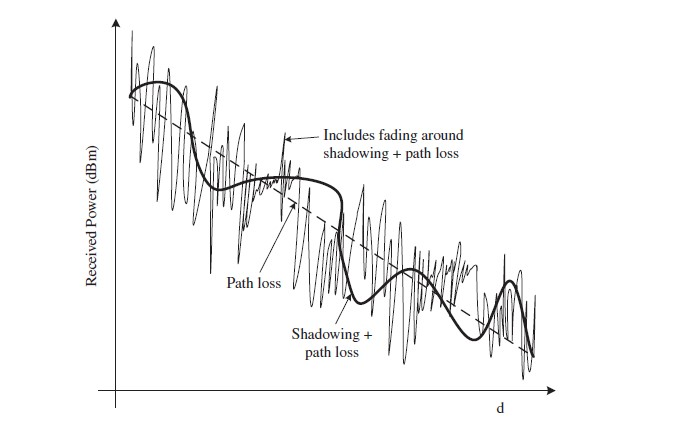
\includegraphics[scale=1]{Chapter 2/Figures/Path Loss}
\caption[Signal Degradation due to Path Loss and Fading]{Variation of Received Signal Power with Distance of separation (d) between transmitter and receiver. Source \textcite{Ghosh2010}}
\label{fig:path loss}
\end{figure}

\section{Diversity}
Mitigation of fading and overcoming low \acrshort{snr} regimes to maintain a suitable \acrshort{qos} requires techniques such as diversity, wherein copies of the same data are sent from the transmitter to the receiver so that reliability of accurately decoding the transmitted symbols is increased.\\
Diversity can be achieved primarily in three ways, they are
\begin{enumerate}
\item \textbf{Frequency Diversity}: Where multiple copies of the same data are sent on different frequency channels
\item \textbf{Time Diversity}: Where multiple copies of the same data are sent at different instances of time
\item \textbf{Spatial Diversity}: Where multiple copies of the same data are sent along different antenna paths.
\end{enumerate}
Among the three possible methods, \gls{spatial diversity} is attractive to us because, the multiple reflections that a signal undergoes in a typical urban setup already provides us with the required diversity without the loss of bandwidth efficiency. Hence, when this report refers to diversity, unless otherwise mentioned, it is assumed to refer to \gls{spatial diversity}. A simplified illustration of multipath propagation in urban setting is shown in the figure \ref{fig:multipath propagation}\\
\begin{figure}[!htbp]
\centering
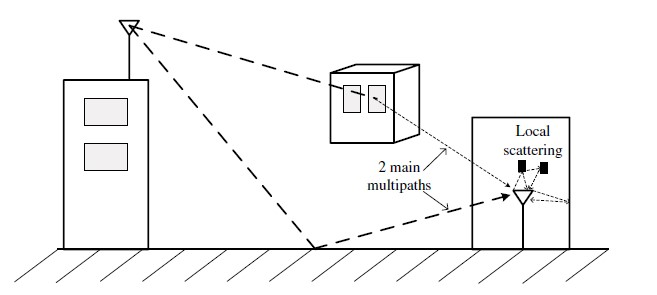
\includegraphics[scale=1]{Chapter 2/Figures/Multipath Propagation}
\caption[Multipath Propagation in a typical urban setting]{Multipath Propagation in a typical urban setting. Source \textcite{Ghosh2010}}
\label{fig:multipath propagation}
\end{figure}
However, in a single channel system, the multiple copies arriving at different time instances leads to interference of the signal. This interference may be constructive or destructive in nature as shown in the figure \ref{fig:constructive and destructive interference}. This can lead to difficulties in decoding as it would mean the requirement of expensive equalizers or reduction in the symbol rate. Neither option is feasible for us, and hence, it becomes apparent to us how having multiple transmit and receive antennas can easily overcome this issue. With the help of multiple antennas, the same situation which was causing \acrlong{isi} (\acrshort{isi}) becomes a boon to us by allowing multiple antenna paths between the transmitter and receiver allowing for easy implementation of \gls{spatial diversity}. This situation is shown in the figure \ref{fig:spatial diversity}\\

\section{Multiplexing}
Supposing the channel conditions are suitable and the \acrshort{snr} is sufficiently high, meaning one is in a high \acrshort{snr} regime, instead of sending multiple copies of the same data, one can send different data blocks on different antenna paths increasing the overall data rate per user and the user capacity of the system. This concept is known as \gls{spatial multiplexing} demonstrated in the figure \ref{fig:spatial multiplexing}.\\

Apart from \gls{spatial multiplexing} one can also implement time multiplexing and frequency multiplexing wherein different data symbols are sent in different time slots or frequency blocks respectively. Modern day \acrshort{4g} and \acrshort{5g} uses all three forms of multiplexing to increase data rates and capacity.\\

When one is given the various options for multiplexing, one can either
\begin{enumerate}
\item Assign multiple resource blocks (either in time, frequency or antenna paths) to a single user to significantly improve his data rate and \acrshort{qos}.
\item The alternative is to accommodate more users by assigning each one or more resource blocks to each and improving the capacity.
\end{enumerate}

This option is left to the service providers to implement resource allocation as per the market requirements. Hence, one sees the significant advantages \acrshort{mimo} has enabled for us by opening the doors to \acrshort{mimo} and \acrshort{mcm}.

\begin{figure}[!htbp]
\centering
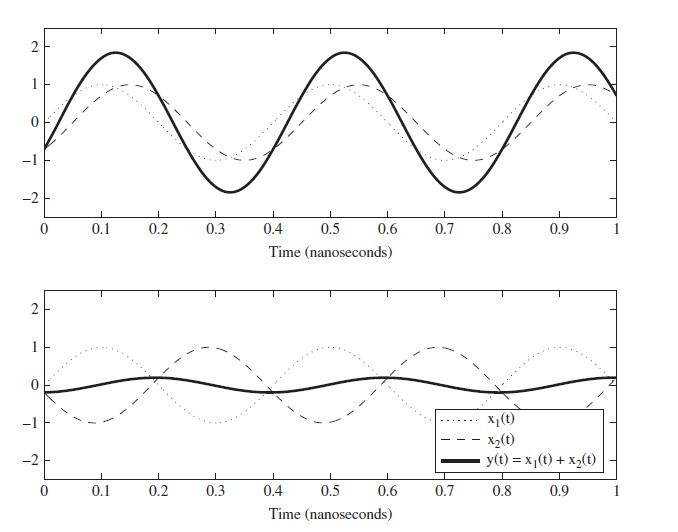
\includegraphics[scale=1]{Chapter 2/Figures/Interference}
\caption[Constructive and Destructive Interference of Signals]{Constructive and Destructive Interference leading to large variation in received signal power. Source \textcite{Ghosh2010}}
\label{fig:constructive and destructive interference}
\end{figure}

\begin{figure}[!htbp]
\centering
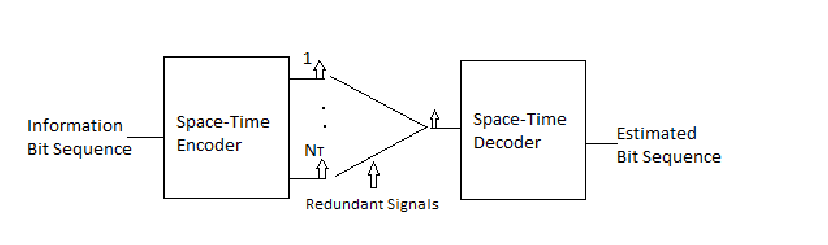
\includegraphics[scale=0.6]{Chapter 2/Figures/Spatial Diversity}
\caption[Spatial Diversity]{Spatial Diversity. Source\textcite{Ghosh2010}}
\label{fig:spatial diversity}
\end{figure}

\begin{figure}[!htbp]
\centering
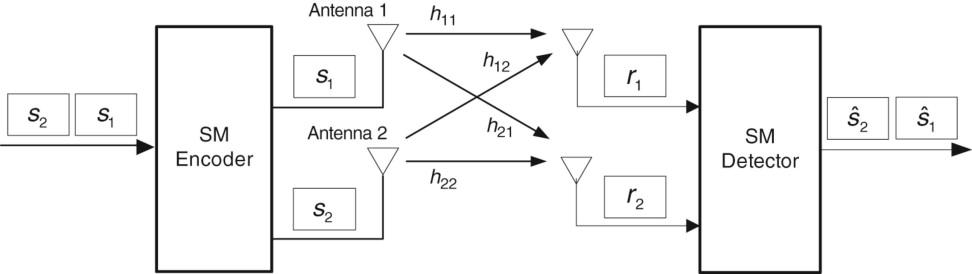
\includegraphics[scale=0.7]{Chapter 2/Figures/Spatial Multiplexing}
\caption{Spatial Multiplexing}
\label{fig:spatial multiplexing}
\end{figure}


\section{Intersymbol Interference, Frequency Selective Fading and the need for MCM}
In the previous section readers saw sufficient motivation to move in the direction of multiple antenna system. However, the issue of \acrshort{isi} needs to be tackled sufficiently to provide significantly high data  rates. Added to the menace of \acrshort{isi} the channel can also degrade the message in a frequency selective manner leading to added difficulties in information recovery at the receiver as shown in the figure \ref{fig:frequency selective fading}. Frequency selective fading occurs because the channel conditions are in constant flux and the message time period is not the same as the time period for which the channel conditions are relatively constant\\
An effective way to combat frequency selective fading is to breakup the entire bandwidth into smaller subchannels where the bandwidth of each subchannel is smaller than the \acrlong{bc} (\acrshort{bc}), thus ensuring that the message time period is smaller than the \acrlong{td} (\acrshort{td}). This approach to communication is called as \acrlong{mcm}(\acrshort{mcm}) technique. The implementation of \acrshort{mcm} is simple if one realizes that one can split the given bandwidth into different subchannels by simply introducing an \acrshort{ifft} block at the transmitter and to achieve the opposite effect introduce an \acrshort{fft} block at the receiver. With the help of this, one is able to significantly reduce the problems of frequency selective fading and \acrshort{isi}. The basic structure of a \acrshort{mcm} transmitter and receiver is given in the figures \ref{fig:mcm transmitter} and \ref{fig:mcm receiver}.

\begin{figure}[!htbp]
\centering
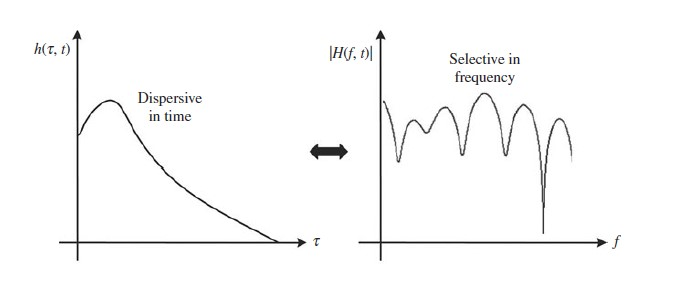
\includegraphics[scale=1]{Chapter 2/Figures/Frequency Selective Fading}
\caption[Frequency Selective Fading]{Frequency Selective Fading which occurs because the message is longer than the delay spread of the channel. Source \textcite{Ghosh2010}}
\label{fig:frequency selective fading}
\end{figure}

\begin{figure}[!htbp]
\centering
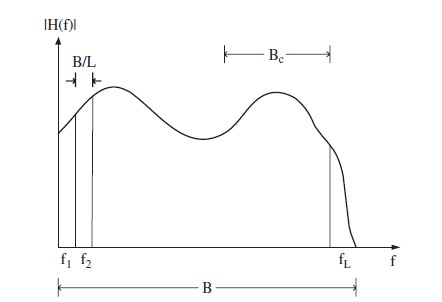
\includegraphics[scale=1]{Chapter 2/Figures/Flat Fading Subchannel}
\caption[Flat Fading Subchannel]{By breaking the large bandwidth into smaller subchannels, one can achieve an almost flat fading subchannel which is desirable. Source \textcite{Ghosh2010}}
\label{fig:flat fading subchannel}
\end{figure}

\begin{figure}[!htbp]
\centering
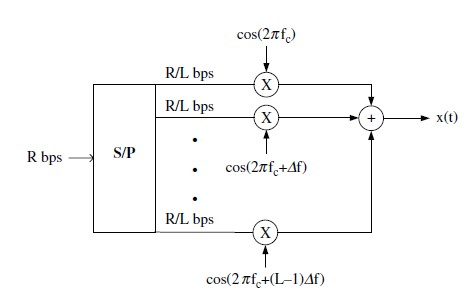
\includegraphics[scale=1]{Chapter 2/Figures/MCM Transmitter}
\caption[MCM Transmitter]{An MCM transmitter with an IFFT block to split the given bandwidth into smaller $L$ subchannels. Source \textcite{Ghosh2010}}
\label{fig:mcm transmitter}
\end{figure}

\begin{figure}[!htbp]
\centering
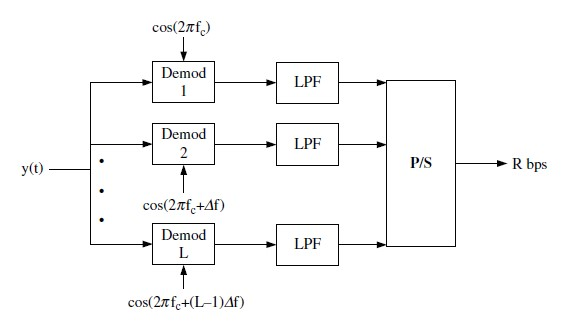
\includegraphics[scale=1]{Chapter 2/Figures/MCM Receiver}
\caption[MCM Receiver]{An MCM transmitter with an FFT block to reverse the effects of IFFT block at the transmitter. Source \textcite{Ghosh2010}}
\label{fig:mcm receiver}
\end{figure}




\section{Shortcomings of simple MCM and the need for OFDM}
Having shown the implementation of a simple \acrshort{mcm} system, this report now addresses some of the shortcomings of this. Primarily,
\begin{itemize}
\item It is impossible to realistically have sharply defined bandwidths, as there exists no way to define a pulse which is strictly rectangular in the frequency domain.
\item Expensive low pass filters will be necessary to maintain orthogonality of the subchannels.
\item Importantly, multiple \acrshort{rf} units are required at both ends for the system to work. This setup, as a result becomes unfeasible and thus, in the next section the reader shall look into the \acrshort{ofdm} scheme as an alternative to simple \acrshort{mcm}.
\end{itemize}

\section{OFDM}
\subsection{Concept of OFDM}
\acrlong{ofdm} is a multiplexing scheme where different data symbols are modulated to different frequencies. These frequencies are chosen such that they are all orthogonal. Hence a given instance, only one wave is at it's peak while the rest are at zero allowing us to read the data bits without any \acrlong{isi}. This situation is shown in the figure \ref{fig:ofdm orthogonal waves}.\\

Therefore, one clubs the different data bits into one block called an \acrshort{ofdm} symbol. To avoid \acrshort{isi} between the \acrshort{ofdm} symbols themselves, there is a small time delay introduced between the \acrshort{ofdm} symbols called as \acrlong{tg} which is abbreviated to \acrshort{tg}. It is important that this delay, is atleast as large as the \acrlong{td}.\\
One knows that the wireless channel behaves as a \acrlong{lti} system and hence, the channel coefficient and data bits are linearly convolved together whenever a message is passed through it. However, one knows that, circular convolution in the time domain yields simple multiplication in the frequency domain. This multiplication is desirable as it leads to simplified computation at the transmitter and receiver. A simple way to covert this linear convolution to circular convolution is to add redundant bits known as \gls{cyclic prefix}. This cyclic prefix is just copying the last $L$ bits of the \acrshort{ofdm} symbol and adding it to the beginning of the symbol. These $L$ bits are transmitted during the time \acrshort{tg} and hence will be lost due to interference between the \acrshort{ofdm} symbols.\\

\begin{figure}[!htbp]
\centering
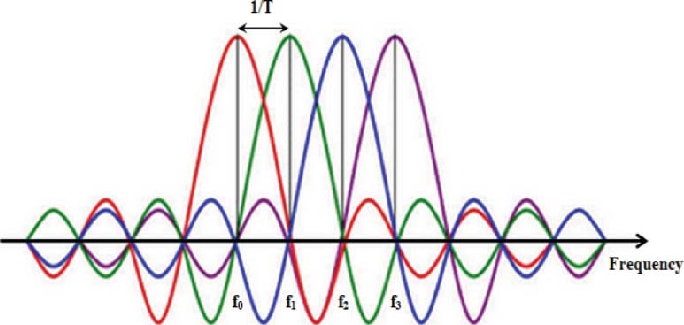
\includegraphics[scale=1]{Chapter 2/Figures/OFDM Orthogonality}
\caption[Orthogonality in OFDM]{An OFDM symbol where different coloured waves correspond to different bits. Notice how when one wave peaks, all the other waves are at their null points. Source \textcite{Ghosh2010}}
\label{fig:ofdm orthogonal waves}
\end{figure}

\begin{figure}[!htbp]
\centering
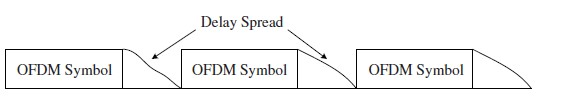
\includegraphics[scale=1]{Chapter 2/Figures/OFDM Symbol Timing}
\caption[Guard Time between OFDM symbols]{A delay of \acrshort{tg} is introduced between the symbols to avoid interference between the \acrshort{ofdm} symbols. Notice that this does not do anything to combat \acrshort{isi} within the \acrshort{ofdm} symbol itself.}
\label{fig:ofdm symbol timing}
\end{figure}

\begin{figure}[!htbp]
\centering
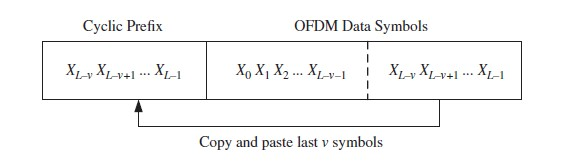
\includegraphics[scale=1]{Chapter 2/Figures/Cyclic Prefix}
\caption[Cyclic Prefix]{The cyclic prefix in an \acrshort{ofdm} symbol. Source \textcite{Ghosh2010}}
\label{fig:ofdm cyclic prefix}
\end{figure}



\subsection{Advantages of OFDM}
Some of the advantages of \acrshort{ofdm} compared to traditional \acrshort{fdm} are as follows.
\begin{itemize}
\item There is no need for any guard bands between carriers leading to higher spectral efficiency.
\item Higher data rates can be achieved as symbol rate need not be lowered for the sake of \acrshort{isi}.
\item System is more robust to multipath effects.
\end{itemize}

\subsection{Disadvantages of OFDM}
\acrshort{ofdm} also comes with a few disadvantages chief among them is the issue of high \acrshort{papr}. Discussing the ways to mitigate this issue is outside the scope of this report and the reader is encouraged to refer to literature such as \textcite{Ghosh2010} to gain a better understanding.

\section{OFDM Transceiver System}
After having seen the motivation for the development of \acrshort{mcm}, \acrshort{mimo} and \acrshort{ofdm} schemes and also having seen a basic \acrshort{mcm} transceiver system, the different concepts are all combined to create an \acrshort{ofdm} transceiver which is capable of sending and receiving data bits packaged in \acrshort{ofdm} symbols.\\
In figure \ref{fig:ofdm transmitter} one can see how normal \acrshort{qam} modulated symbols are passed through an \acrshort{ifft} block to assign them to different frequency subchannels. Additional cyclic prefix is added before converting the parallel streams to a serial stream and transmitting it.\\
The \acrshort{ofdm} receiver in figure \ref{fig:ofdm receiver} on the other hand does the exact opposite process, where the received symbols are demodulated according to their respective frequencies and passed through an \acrshort{fft} block to undo the \acrshort{ifft} process. Then, it the demodulated symbols are passed through a \acrlong{mli} detector to get back the information bits.\\

\begin{figure}[!htbp]
\centering
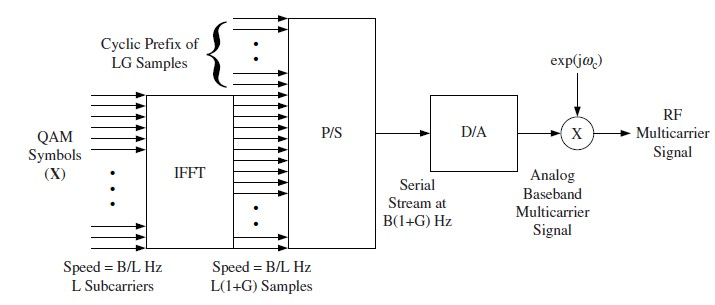
\includegraphics[scale=1]{Chapter 2/Figures/OFDM Transmitter}
\caption[\acrshort{ofdm} Transmitter]{\acrshort{ofdm} Transmitter. Source \textcite{Ghosh2010}}
\label{fig:ofdm transmitter}
\end{figure}

\begin{figure}[!htbp]
\centering
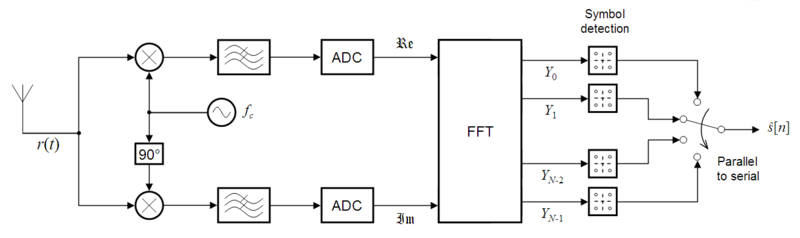
\includegraphics[scale=0.6]{Chapter 2/Figures/OFDM Receiver}
\caption[\acrshort{ofdm} Receiver]{\acrshort{ofdm} Receiver. Source \textcite{Ghosh2010}}
\label{fig:ofdm receiver}
\end{figure}


\section{Alamouti Coding Scheme}
Alamouti coding scheme is a simple coding scheme designed for the purpose of achieving \gls{spatial diversity} in \acrshort{miso} systems. The advantage of this coding scheme is that the transmitter need not know the channel information before sending the data. This section describes the coding scheme.\\
Consider two transmitting antennas $T_1$ and $T_2$ and one receiving antenna $R$.\\
Let $h_1$ be the channel coefficient of the first antenna path and $h_2$ be the channel coefficient of the second antenna path.\\
Let $x_1$ and $x_2$ be transmitted by antennas $T_1$ and $T_2$ respectively at a given time instance, and ${-x_2}^*$, ${-x_1}^*$ be the data transmitted in the next time instance by the antennas respectivey.\\
It is known that the wireless channel behaves as an \acrshort{lti} system which performs convolution of the data bits and the channel coefficient. Also, let $w_1$ and $w_2$ be the noise vectors added at the two time instances respectively.\\
This situation can be represented mathematically as follows.
\begin{align}
y_1 &= 
\begin{bmatrix}
h_1&h_2
\end{bmatrix}
\times
\begin{bmatrix}
x_1\\
x_2
\end{bmatrix}
+ w_1\\
y_2 &=
\begin{bmatrix}
h_1&h_2
\end{bmatrix}
\times
\begin{bmatrix}
{-x_2}^*\\
x_1^*
\end{bmatrix}
+w_2
\end{align}
This can be further simplified as,\\
\begin{align}
y &= \begin{bmatrix}
y_1\\
y_2^*
\end{bmatrix}
= c_1x_1 + c_2x_2 + w
\end{align}
Where,
\begin{align}
c_1&=\begin{bmatrix}
h_1\\
h_2^*
\end{bmatrix}\\
c_2&=\begin{bmatrix}
h_2\\
-h_1^*
\end{bmatrix}
\end{align}
Here $c_1$ and $c_2$ can be shown as orthogonal in nature and so, this coding scheme is also known as \acrlong{ostbc} scheme.\\
At the receiver, once the matrix $y$ is obtained, $x_1$ and $x_2$ can be recovered as follows,
\begin{align}
\frac{c_1^H}{||c_1||} \cdot y &= ||c_1||x_1 + \overline{w_1}\\
\frac{c_2^H}{||c_2||} \cdot y &= ||c_2||x_2 + \overline{w_2}
\end{align}
Here, $c_1^H$ and $c_2^H$ are the result obtained after performing the Hermitian operator on the $c$ matrices. It is noticed that $x_1$ and $x_2$ are scaled by a factor and mixed with \acrshort{awgn} noise. With a suitable decision criteria, both $x_1$ and $x_2$ can be decoded correctly in two time slots. This shows how Alamouti coding scheme is effective when used in the \gls{spatial diversity} mode of a $2 \times 1$ \acrshort{miso} system. However, in higher order schemes, Alamouti coding loses it's efficiency and is not feasible.

\section{Inverse Channel Estimation}
The received symbol vector $y$ is related to the transmitted vector $x$ and channel coefficient matrix $h$ as\\
\begin{align}
\begin{bmatrix}
y
\end{bmatrix}
&=
\begin{bmatrix}
x
\end{bmatrix}
\times
\begin{bmatrix}
h
\end{bmatrix}
+
\begin{bmatrix}
n
\end{bmatrix}
\end{align}
where $\begin{bmatrix} n \end{bmatrix}$ is the \acrshort{awgn} noise vector.\\
From this, one can extract the sent symbols by multiplying $\begin{bmatrix} y \end{bmatrix}$ with the inverse of the channel coefficient matrix which yields the following expression.

\begin{align}
\begin{bmatrix}
y
\end{bmatrix}
\times
\begin{bmatrix}
h
\end{bmatrix}
^{-1}
&=
\begin{bmatrix}
x
\end{bmatrix}
+
\begin{bmatrix}
w_1
\end{bmatrix}
\end{align}
where $\begin{bmatrix} w_1 \end{bmatrix}$ is the result obtained after multiplying $\begin{bmatrix} n \end{bmatrix}$ with $\begin{bmatrix}h \end{bmatrix}^{-1}$.\\

Further processing is necessary to remove the noise vector $\begin{bmatrix} w_1 \end{bmatrix}$. However, one of the issues that us faced is that $\begin{bmatrix} w_1 \end{bmatrix}$ is no longer \acrshort{awgn} but becomes colored noise. Therefore, to overcome this hindrance,  precoding of the transmitted symbols vector $\begin{bmatrix} x \end{bmatrix}$ is done by multiplying it with $\begin{bmatrix} h \end{bmatrix}^{-1}$. The received vector $\begin{bmatrix} y \end{bmatrix}$ then becomes

\begin{align}
\begin{bmatrix} y \end{bmatrix} &=
\begin{bmatrix} x \end{bmatrix}
\times
\begin{bmatrix} h \end{bmatrix}^{-1}
+
\begin{bmatrix} n \end{bmatrix}
\end{align}

Finally, when one tries and extracts the transmitted symbols at the receiver by multiplying with $\begin{bmatrix} h \end{bmatrix}$ one gets

\begin{align*}
\begin{bmatrix} y \end{bmatrix} \times
\begin{bmatrix} h \end{bmatrix} &=
\times
\begin{bmatrix} x \end{bmatrix}
+
\begin{bmatrix} w_2 \end{bmatrix}
\end{align*}
where $\begin{bmatrix} w_2 \end{bmatrix}$ is the result obtained after multiplying $\begin{bmatrix} n \end{bmatrix}$ with $\begin{bmatrix} h \end{bmatrix}$.\\

Now, $\begin{bmatrix} w_2 \end{bmatrix}$ remains to be Gaussian and hence further noise processing becomes simpler with normal demodulators and \acrshort{mli} estimators.




\section{Singular Value Decomposition}
In the previous section readers saw the advantage of using Inverse Channel Estimation precoding. However, in massive \acrshort{mimo} systems where the number of antenna paths are plenty and the order of the channel coefficient matrix is large, inversion of matrices becomes a computationally intensive task. Since it is required to have high speed \gls{modems} which do not take more than a few microseconds to make the necessary computations, one must look to faster ways of inverting the channel coefficient matrix.\\
In this effort this report uses the singular value decomposition technique where one decomposes the channel coefficient matrix $\begin{bmatrix} h \end{bmatrix}$ into three orthogonal matrices $\begin{bmatrix} U \end{bmatrix}$ , $\begin{bmatrix} \Sigma \end{bmatrix}$ and, $\begin{bmatrix} V \end{bmatrix}$.

At the transmitter one multiplies the transmitted symbol vector $\begin{bmatrix} x \end{bmatrix}$ with $\begin{bmatrix} V \end{bmatrix}$ and similarly at the receiver one multiplies the received vector $\begin{bmatrix} y \end{bmatrix}$ with $\begin{bmatrix} U \end{bmatrix}$ to achieve the same effect as inversion.\\
Singular value decomposition is faster than regular inversion for large matrices and hence proves faster in massive \acrshort{mimo} systems.

\section*{Summary}
This chapter has elaborated on the motivations behind \acrshort{mcm} and \acrshort{mimo}. The authors have also clearly elaborated on the key technologies that enable them. The next chapter discusses the implementation details of the \acrshort{mcm}-\acrshort{mimo} system and explains the different algorithms used. Finally, in Chapter 4 the results obtained after simulations are discussed and conclusions are drawn as to the overall system performance.  


%Chapter 3 Design Methodology
\chapter{Design of MCM and MIMO Processing Systems for Urban Communication}

The focus here is primarily on the algorithms implemented as part of the \acrshort{mcm}-\acrshort{mimo} system. The different aspects of transmitter block, channel parameters and receiver block of the system are looked into. The simulations of \acrshort{siso}, \acrshort{simo} ( transmit \gls{spatial diversity}), \acrshort{miso} (\acrshort{ostbc}) and \acrshort{mimo} ( both \gls{spatial diversity} and multiplexing(inverse channel decoding and \acrshort{svd})) are also looked into.
 
\section{Basic Overview of our System}

Figure \ref{fig:general block digram} shows the general block diagram of a communication system, similar to the one mentioned in Chapter 1.
In the following sections the discussion is on the role of each block in detail by building on the foundation laid in the previous chapters.

\begin{figure}[!htbp]
\centering
\includegraphics[scale=0.8]{Chapter 3/Figures/Wireless Communication System Block Diagram}
\label{fig:general block digram}
\caption{General Wireless Communication System Block Diagram}
\end{figure}

\section{Transmitter}

The various sections of the transmitter block are explored in the beginning. There is no concern with the source information as they are just randomized binary digits generated by the \gls{matlab} rand function. Neither is there any concern with the \acrlong{dac}(\acrshort{dac}) as it is beyond the scope of this report.\\

Instead, the focus is on the \acrshort{qam} modulator and various precoders which work on the principles explained in Chapter 2. The section also looks into the \acrlong{prbs}(\acrshort{prbs}) generator which is used for channel estimation and the tone loading algorithm which is employed in the cases of \acrshort{siso}, \acrshort{simo} and \acrshort{mimo} both in diversity and multiplexing cases.

\subsection{PRBS Generator}
A good \acrlong{prbs} generator is key for generating the pilot signals which is needed for the modem training phase and channel characteristic estimation. For these purposes our system uses the \acrshort{prbs} generator algorithm presented in \textcite{ITU2009} which is defined below.

The $n^{th}$ pseudo random binary digit $d_n$ is given by 

\begin{align*}
d_n &= 1 & \text{for n = 1 to 9}\\
d_n &= d_{n-4} \oplus d_{n-9} & \text{for n = 10 to 2 $\times$ NSC}\\
d_n &= d_{n-2 \times NSC} & \text{for n = 2 $\times$ NSC + 1 to 2 $\times$ NSC + 2}\\
d_n &= d_{4 \times NSC +2 -n} & \text{for n = 2 $\times$ NSC + 3 to 4 $\times$ NSC (n odd)}\\
d_n &= 1 \oplus d_{4 \times NSC +4 -n} & \text{for n = 2 $\times$ NSC + 3 to 4 $\times$ NSC (n even)}
\end{align*}
Here \acrshort{nsc} is the total number of subcarriers, taken to be 256 in our case. Hence, upto 1024 \acrshort{prbs} digits can be generated. However, the limit is set to the first 512 digits only as 2 bits is allocated per channel.

\subsection{Tone Loading Algorithm for the transmitter}
Once the channel conditions are determined by transmitting the pilot signals and the \acrshort{snr} of each subchannel is measured to create a channel profile, it becomes necessary to load the data bits onto these subchannels in an efficient manner. Common sense tells us that the subchannels with higher \acrshort{snr} should carry more bits than those with lower \acrshort{snr}. It is shown through the tone loading algorithm that this is indeed the case.\\
The basis for our tone loading algorithm is the capacity law given by Shannon in \textcite{Shannnon1948}. Using this formula, the number of bits that a given subchannel can support for it's given \acrshort{snr} is determined. Then, the number of bits is rounded and the power deviation is calculated. Finally, the bit loading profile is obtained by applying the inverse of the capacity law. As long as this deviation is within the agreed upon threshold, addition and removal of bits between the subchannels until a stable tone loading situation arises is done.\\
The limit set for the purposes of this is $\pm 2$ dB and an additional constraint of setting the maximum number of bits for any channel to be 20 is addeds. The exact details of the algorithm is given in Algorithm \ref{alg:Fine Gains Algorithm}.

\begin{algorithm}[!htbp]
\caption{Fine Gains Tone Loading Algorithm}
\label{alg:Fine Gains Algorithm}
\begin{algorithmic}
\STATE {$b_i \gets log_2(1+SNR_i)$}\\
\STATE {$\hat{b}_i \gets \nint{b_i}$}\\
\STATE {$\delta_i \gets b_i - \hat{b}_i$}\\
\STATE {$P_{\delta_i} \gets 3 \times \delta_i$}\\
\STATE {$P_{\delta_{total}} \gets \sum_{i=1}^{NSC} P_{\delta_i}$}\\
\WHILE {$P_{\delta_{total}} > P_{threshold} \OR P_{\delta_{total}} < -P_{threshold}$}
	\IF {$P_{\delta_{total}} > P_{threshold}$}
		\STATE {$position=\verb|POS|(\verb|MAX|(\delta_i))$}\\
		\STATE {$\hat{b}_{position} \gets \hat{b}_{position} - 1 $}\\
		\STATE {$\delta_{position} \gets b_{position} - \hat{b}_{position}$}\\
		\STATE {$P_{\delta_{position}} \gets 3 \times \delta_{position}$}\\
		\STATE {$P_{\delta_{total}} \gets \sum_{i=1}^{NSC} P_{\delta_i}$}\\
	\ELSIF {$P_{\delta_{total}} < -P_{threshold}$}
		\STATE {$position=\verb|POS|(\verb|MIN|(\delta_i))$}\\
		\STATE {$\hat{b}_{position} \gets \hat{b}_{position} + 1 $}\\
		\STATE {$\delta_{position} \gets b_{position} - \hat{b}_{position}$}\\
		\STATE {$P_{\delta_{position}} \gets 3 \times \delta_{position}$}\\
		\STATE {$P_{\delta_{total}} \gets \sum_{i=1}^{NSC} P_{\delta_i}$}\\
	\ENDIF
\ENDWHILE
\STATE {$SNR_i \gets 2^{\hat{b}_i}-1$} 
\end{algorithmic}
\end{algorithm}

\subsection{QAM Modulator}
Among the various modulation schemes available for us, the choice of \acrshort{qam} modulation technique is done because it is extremely power efficient and also maintains a good degree of spectral efficiency.\\

One of the problems the system runs into with \acrshort{qam} modulation is the fact that there is a need to maintain large symbol constellations, especially when there are with higher order \acrshort{qam} modulation schemes to be considered. Therefore, a fast recursive algorithm that can generate large symbol constellations by keeping only a few small constellations in memory is discussed. This approach reduces the cost of hardware required by reducing the memory elements required but still maintains a high degree of speed. The details of this are given in \ref{alg:Working of Modulator}

\begin{algorithm}[!htbp]
\caption{Bits to Constellation Mapping Algorithm}
\label{alg:Working of Modulator}
\begin{algorithmic}
\STATE {$LUT \gets \verb|{QAM_1, QAM_2, QAM_3, QAM_5}|$}
\STATE {$matrix_{transform} \gets \verb|{0, -2i, 2, 2+2i}|$}
\STATE {$i \gets 1$}
\WHILE {$i < NSC $}
	\STATE {$flag_{recursion} \gets \FALSE$}
	\IF {$b_i == 1$}
		\STATE {$symbol_i \gets \verb|QAM_1|(bits_i)$}
	\ELSIF {$b_i \% 2 == 0 \quad \AND \quad b_i \quad \NOT = 0$}
		\STATE {$bits_{extracted} \gets$ extract $bits$ into groups of 2}
		\STATE {$bits_{decimal} \gets \texttt{DEC}(bits_{extracted})$}
		\STATE {$symbol_i \gets \verb|QAM_2|(bits_{decimal})$}
		\STATE {$flag_{recursion} \gets \TRUE$}
	\ELSIF {$b_i \% 2 == 1$}
		\STATE {$symbol_i \gets \verb|QAM_3|(bits_i)$}
		\IF {$b_i > 3$}
			\STATE {$bits_{extracted} \gets$ Extract bits into groups of 2}
			\STATE{$bits_{decimal} \gets \texttt{DEC}({bits_{extracted}})$}
			\IF {$bits_{decimal} < 4$}
				\STATE {$symbol_i \gets \verb|QAM_3|(bits_{decimal})$}
			\ELSE
				\STATE {$symbol_i \gets \verb|QAM_5|(bits_{decimal})$}
			\ENDIF
			\STATE{$flag_{recursion} \gets \TRUE$}
		\ENDIF
	\ENDIF
	\IF {$flag_{recursion}$}
		\STATE {$count = 2$}
		\WHILE {$count < \texttt{SIZE}(bits_{decimal})$}
			\STATE {$bits_{decimal_{extracted}} \gets $ Extract the bits individually}
			\STATE {$point_{quadrant} \gets \texttt{GET BASIC QUADRANT POINT}$}
			\STATE {$offset \gets \texttt{FIND OFFSET(}point_{quadrant} , bits_{decimal_{extracted}})$}
			\STATE {$symbol_i \gets 2 \times symbol_i - \verb|QAM_2|(bits_{decimal_{extracted}}) + point_{quadrant} + offset$}
			\STATE {$count \gets count + 1$}
		\ENDWHILE
	\ENDIF
	\STATE {$i \gets i +1$}
\ENDWHILE
\end{algorithmic}
\end{algorithm} 




\section{Channel Parameters}
The transmitter portion of the system was discussed earlier, now emphasis is on the channel parameters which are mostly randomized in nature. The various channel parameters like noise, fading and path loss are discussed in the following paragraphs.

\subsection{AWGN Noise}
All communication is affected by noise, the assumption here is that \acrlong{awgn} noise is the noise function of choice. To generate this, the \gls{matlab} function \emph{randn} is used which generates a Gaussian function with mean as $0$ and variance as $1$. Then this function is multiplied with the noise variance of our choice to get the noise signal. Mathematically, \acrshort{awgn} function is given by 
\begin{align}
noise&= \frac{1}{\sqrt{2\pi\sigma^2}}e^{\frac{x^2}{2\sigma^2}}
\end{align}

Where $\sigma$ is the noise variance or power. In \gls{matlab}, this is given by the statement
\begin{verbatim}
noise = sqrt(noise_power_abs/2) .* ((randn(Nsc,1)) + 1i*randn(Nsc,1));
\end{verbatim}
Here, \acrshort{nsc} is the \acrlong{nsc}. Since the attempt is to add noise to all the subchannels, the vector is of the size $\acrshort{nsc} \times 1$.

\subsection{Rayleigh Fading}
Earlier, fading in wireless channels was mentioned. It was also mentioned that \gls{rayleigh fading} was the model of choice for our report. \gls{rayleigh fading} is viewed as a reasonable model for tropospheric and ionospheric propagation as well as for heavy urban settings for wireless signals. \gls{rayleigh fading} is most applicable when there is no dominant propagation along a line of sight between the transmitter and receiver. \gls{rayleigh fading} is any function that varies as per the Rayleigh distribution which is the radial component of the sum of two uncorrelated Gaussian random variables. In \gls{matlab} this is generated through,
\begin{verbatim}
rayleigh_channel = sqrt(1/2) .* (randn(1) + 1i*randn(1))
\end{verbatim}
where the two \emph{randn} functions produce the two uncorrelated Gaussian functions.

\subsection{Path Loss Function}
Path loss function determine the way in which the transmitted signal degrades with distance before the signal reaches the receiver. Since the focus is on \acrlong{los} path propagation \acrshort{los} path loss formulation as given by Friis Transmission formula is considered.
\begin{align}
P_r &= \frac{P_t G_t G_r \lambda^2}{(4 \pi r)^2} 
\end{align}
where:

\begin{align*}
P_r &= \text{Received Signal Power}\\
P_t &= \text{Transmitted Signal Power, in our simulations it is 1 mW}\\
G_t &= \text{Transmitter Antenna Gain, in our simulations it is 8}\\
G_r &= \text{Receiver Antenna Gain, in our simulation it is 1}\\
r &= \text{Distance of separation between the two antennas, in our simulations it is 1 Km}\\
\lambda &= \text{Wavelength of the signal wave}.\\
\end{align*}


\section{Receiver}
The receiver the system employs consists of an estimator, decoder and demodulator. The estimator uses the principle of maximum likelihood estimation. In \acrshort{mli} at the receiver the received symbol is taken and plotted as a point on the symbol constellation. Then, the Euclidian distance of this point from all the constellation points is calculated and the constellation point whose Euclidian distance is closest to the received symbol point is chosen. This technique is optimal and gives the least amount of error thereby improving the system performance.\\

The decoders like Alamouti decoder and \acrshort{svd} decoder have already been discussed in the previous chapter.

Our estimator system also works on a similar principle but makes use of the unique constellation mapping algorithm to greatly simplify the decision making process by following Algorithm \ref{alg:Working of Estimator}.\\

Once the estimator has estimated a constellation point for us, the demodulator converts this constellation point into the binary digits representing the constellation point. Similar to the case of modulation, all the constellations are not stored in memory but generated dynamically using a recursive algorithm. This process is shown in Algorithm \ref{alg:Working of Demodulator} 

\begin{algorithm}[!htbp]
\caption{Estimation Algorithm}
\label{alg:Working of Estimator}
\begin{algorithmic}
\STATE {$LUT \gets \verb|{QAM_1, QAM_2, QAM_3}|$} 
\STATE {$i \gets 1$}
\WHILE {$i < NSC $}
	\IF {$b_i == 0$}
		\STATE {$estimate_i \gets 0$}
	\ELSIF {$b_i == 1$}
		\STATE {$estimate_i \gets \verb|CLOSEST|(\verb|QAM1|, received_i)$}
	\ELSIF {$b_i == 3$}
		\STATE {$estimate_i \gets \verb|CLOSEST|(\verb|QAM_3|, received_i)$}
	\ELSIF {$b_i \geq 2$}
		\STATE {$real_i \gets \floor{\texttt{REAL}(received_i)}$}
		\STATE {$imag_i \gets \floor{\texttt{IMAG}(received_i)}$}
		\IF{$real_i \% 2 ==0$}
			\STATE {$real_i = real_i +1$}
		\ENDIF
		\IF{$imag_i \% 2 ==0$}
			\STATE {$imag_i = imag_i +1$}
		\ENDIF
		\STATE {$estimate_i \gets real_i + imag_i$}
		\STATE {$estimate_i \gets \verb|BOUND TO MAX|(estimate_i)$} 
	\ENDIF
	\STATE {$i \gets i +1$}
\ENDWHILE
\end{algorithmic}
\end{algorithm} 

\begin{algorithm}[!htbp]
\caption{Constellation to Bits Mapping Algorithm}
\label{alg:Working of Demodulator}
\begin{algorithmic}
\STATE {$LUT \gets \verb|{QAM_1, QAM_2, QAM_3, QAM_5}|$}
\STATE {$matrix_{transform} \gets \verb|{0, -2i, 2, 2+2i}|$}
\STATE {$i \gets 1$}
\WHILE {$i < NSC $}
	\IF {$b_i == 1$}
		\STATE {$symbol_i \gets \texttt{BIN(FIND}(estimate_i, \verb|QAM_1|))$}
	\ELSIF {$b_i == 3$}
		\STATE {$symbol_i \gets \texttt{BIN(FIND}(estimate_i, \verb|QAM_3|))$}
	\ELSIF {$b_i \geq 2$}
		\STATE {$symbol_i \gets \texttt{NULL}$}
		\IF {$b_i \% 2 == 0$}
			\STATE {$limit \gets \frac{b_i}{2} -1$}
		\ELSE
			\STATE {$limit \gets \frac{b_i-3}{2} -1$}
		\ENDIF
		\STATE {$point_{quadrant} \gets \texttt{GET BASIC QUADRANT POINT}$}
		\STATE{$count \gets 1$}
		\WHILE{$count < limit$}
			\STATE{$offset \gets \texttt{FIND OFFSET(}point_{quadrant} , estimate_i)$}
			\STATE {$value_{binary} \gets \texttt{BIN(FIND(}offset, matrix_{transform}))$}
			\STATE {$symbol_i \gets symbol_i + value_{binary}$}
			\STATE{$estimate_i \gets \frac{estimate_i}{2}$}
			\STATE{$count \gets count +1$}
		\ENDWHILE
	\ENDIF
	\STATE {$i \gets i +1$}
\ENDWHILE
\end{algorithmic}
\end{algorithm} 



\section{Operation of the System in Different Modes}
The various modes in which our system can be operated are discussed here. The algorithm that the system follows in each mode is described in detail here. In some cases like \acrshort{mimo} it is possible to operate the system with various precoders and hence this section discusses in detail these algorithms as well.

\subsection{SISO Mode}
In the \acrlong{siso} mode, only one antenna each is present at both the transmitter and receiver. The steps involved in sending the data from transmitter to the receiver in the \acrshort{siso} is given in Algorithm \ref{alg:Operation in SISO Mode}.

\begin{algorithm}[!htbp]
\caption{Operation in SISO Mode}
\label{alg:Operation in SISO Mode}
\begin{enumerate}
\item Get pilot signals through the PRBS Generator
\item Get QAM symbols by modulating the pilot bits with the modulator
\item Obtain the Rayleigh channel coefficient
\item Obtain the received power with the help of LOS function
\item Generate the noise signal
\item Determine the channel coefficient as $h \gets \sqrt{\frac{P_r}{P_t}} \times rayleigh$
\item Send the pilot signals from transmitter to the receiver
\item Get the received pilot symbols by doing $symbol_{received} \gets symbol_{sent} \times h$
\item Estimate the \acrshort{snr} of the subchannels with the help received power
\item Estimate the value of channel coefficients at the receiver with the help of received pilot signals
\item Get the data bits and modulate them into \acrshort{qam} symbols
\item Perform tone loading with the help of fine gains algorithm
\item Send the data \acrshort{qam} symbols as per the tone loading profile
\item Add noise signal and multiply data signal with channel coefficients to simulate path loss and fading
\item Demodulate the received data symbols with the help of estimated channel coefficients at the receiver
\item Use a \acrlong{mli} to determine the sent bits
\item Calculate the \acrshort{ber} for the system
\end{enumerate}
\end{algorithm} 


\subsection{SIMO System}
In the \acrlong{simo} mode, only one antenna is present at the transmitter but there are 2 antennas at the receiver leading to 2 possible antenna paths. The steps involved in sending the data from transmitter to the receiver in the \acrshort{simo} is given in Algorithm \ref{alg:Operation in SIMO Mode}.

\begin{algorithm}[!htbp]
\caption{Operation in SIMO Mode}
\label{alg:Operation in SIMO Mode}
\begin{enumerate}
\item Get pilot signals through the PRBS Generator
\item Get QAM symbols by modulating the pilot bits with the modulator
\item Obtain both the Rayleigh channel coefficient
\item Obtain the received power with the help of LOS function for both paths
\item Generate the noise signal
\item Determine both the channel coefficients as $h_i \gets \sqrt{\frac{P_{r_i}}{P_{t_i}}} \times rayleigh_i$
\item Send the pilot signals from transmitter to the receiver in both paths
\item Get the received pilot symbols for both paths by doing $symbol_{received} \gets symbol_{sent} \times h_i$
\item Estimate the \acrshort{snr} of the subchannels for both paths with the help received power
\item Estimate the value of channel coefficients for both paths at the receiver with the help of received pilot signals
\item For each subchannel choose the optimal antenna path between the two possibilities
\item Get the data bits and modulate them into \acrshort{qam} symbols
\item Perform tone loading with the help of fine gains algorithm for the optimal data paths
\item Send the data \acrshort{qam} symbols as per the tone loading profile in the optimal data paths
\item Add noise signal and multiply data signal with respective channel coefficient to simulate path loss and fading
\item Demodulate the received data symbols with the help of estimated channel coefficient of the path in which data was received at the receiver
\item Use a \acrlong{mli} to determine the sent bits
\item Calculate the \acrshort{ber} for the system
\end{enumerate}
\end{algorithm} 

\subsection{MISO System}
In the \acrlong{miso} mode, only one antenna is present at the receiver but there are 2 antennas at the transmitter leading to 2 possible antenna paths. The steps involved in sending the data from transmitter to the receiver in the \acrshort{miso} is given in Algorithm \ref{alg:Operation in MISO Mode}.

\begin{algorithm}[!htbp]
\caption{Operation in MISO Mode}
\label{alg:Operation in MISO Mode}
\begin{enumerate}
\item Get pilot signals through the PRBS Generator
\item Get QAM symbols by modulating the pilot bits with the modulator
\item Obtain both the Rayleigh channel coefficient
\item Obtain the received power with the help of LOS function for both paths
\item Generate the noise signal
\item Determine both the channel coefficients as $h_i \gets \sqrt{\frac{P_{r_i}}{P_{t_i}}} \times rayleigh_i$
\item Send the pilot signals from transmitter to the receiver in both paths
\item Get the received pilot symbols for both paths by doing $symbol_{received} \gets symbol_{sent} \times h_i$
\item Estimate the value of channel coefficients for both paths at the receiver with the help of received pilot signals
\item Get the data bits and modulate them into \acrshort{qam} symbols
\item Perform Alamouti Coding and send the data symbol and the conjugate data symbol in alternate cycles and alternate paths as described in Alamouti Coding Scheme
\item Add noise signal and multiply data signal with respective channel coefficient to simulate path loss and fading
\item Demodulate the received data symbols with the help of estimated channel coefficient of the path in which data was received at the receiver
\item Perform Alamouti decoding as previously described to get 2 data symbols in 2 consecutive cycles
\item Use a \acrlong{mli} to determine the sent bits
\item Calculate the \acrshort{ber} for the system
\end{enumerate}
\end{algorithm} 

\subsection{MIMO System}
In the \acrlong{mimo} mode, 2 antennas are present at both the receiver and the transmitter leading to 4 possible antenna paths. This also affords us the option of whether the system is to be used in diversity mode or multiplexing mode depending on the channel conditions.\\
If the channel being operated in has low \acrshort{snr} characteristics, the system is operated in the diversity mode. The steps involved in sending the data from transmitter to the receiver in the \acrshort{mimo} diversity mode is given in Algorithm \ref{alg:Operation in MIMO Diversity Mode}.\\
However, supposing there exists a sufficiently high \acrshort{snr}, the system can then operate in the multiplexing mode. The steps involved in operating the system in \acrshort{mimo} multiplexing mode are given in Algorithm \ref{alg:Operation in MIMO Multiplexing Mode}.\\

For the multiplexing mode again, there exists different precoding options like Inverse Channel Estimation Precoding and \acrlong{svd} precoding. These techniques have already been discussed in the previous chapter and the algorithm for implementation are provided here. Algorithm \ref{alg:Operation in MIMO Inverse Channel Estimation Mode} provides the details of operating the system with an Inverse Channel Estimator and Algorithm \ref{alg:Operation in MIMO SVD Mode} provides the details for operating the system with a \acrshort{svd} precoder.\\

\begin{algorithm}[!htbp]
\caption{Operation in MIMO Diversity Mode}
\label{alg:Operation in MIMO Diversity Mode}
\begin{enumerate}
\item Get pilot signals through the PRBS Generator
\item Get QAM symbols by modulating the pilot bits with the modulator
\item Obtain all the Rayleigh channel coefficients
\item Obtain the received power with the help of LOS function for all  paths
\item Generate the noise signal
\item Determine all the channel coefficients as $h_i \gets \sqrt{\frac{P_{r_i}}{P_{t_i}}} \times rayleigh_i$
\item Send the pilot signals from transmitter to the receiver in all paths
\item Get the received pilot symbols for all paths by doing $symbol_{received} \gets symbol_{sent} \times h_i$
\item Estimate the \acrshort{snr} of the subchannels with the help received power
\item Estimate the value of channel coefficients for all paths at the receiver with the help of received pilot signals
\item For each subchannel choose the optimal antenna path between the four possibilities
\item Get the data bits and modulate them into \acrshort{qam} symbols
\item Perform tone loading with the help of fine gains algorithm for the optimal data paths
\item Add noise signal and multiply data signal with respective channel coefficient to simulate path loss and fading
\item Demodulate the received data symbols with the help of estimated channel coefficient of the path in which data was received at the receiver
\item Use a \acrlong{mli} to determine the sent bits
\item Calculate the \acrshort{ber} for the system
\end{enumerate}
\end{algorithm} 

\begin{algorithm}[!htbp]
\caption{Operation in MIMO Multiplexing Mode}
\label{alg:Operation in MIMO Multiplexing Mode}
\begin{enumerate}
\item Get pilot signals through the PRBS Generator
\item Get QAM symbols by modulating the pilot bits with the modulator
\item Obtain all the Rayleigh channel coefficients
\item Obtain the received power with the help of LOS function for all  paths
\item Generate the noise signal
\item Determine all the channel coefficients as $h_i \gets \sqrt{\frac{P_{r_i}}{P_{t_i}}} \times rayleigh_i$
\item Send the pilot signals from transmitter to the receiver in all paths
\item Get the received pilot symbols for all paths by doing $symbol_{received} \gets symbol_{sent} \times h_i$
\item Estimate the \acrshort{snr} of the subchannels with the help received power
\item Estimate the value of channel coefficients for all paths at the receiver with the help of received pilot signals
\item For transmitting antenna $T_1$ choose the optimal channel path from the two available paths. Similarly, for $T_2$ choose an optimal path from the two available paths.
\item Get the data bits and modulate them into \acrshort{qam} symbols
\item Perform tone loading for $T_1$ and $T_2$ onto their respective optimal channels with the help of fine gains algorithm
\item Add noise signal and multiply data signal with respective channel coefficient to simulate path loss and fading
\item Demodulate the received data symbols with the help of estimated channel coefficient of the path in which data was received at the receiver
\item Use a \acrlong{mli} to determine the sent bits
\item Calculate the \acrshort{ber} for the system
\end{enumerate}
\end{algorithm}

\begin{algorithm}[!htbp]
\caption{Operation in MIMO Multiplexing Mode with Inverse Channel Estimation Precoding}
\label{alg:Operation in MIMO Inverse Channel Estimation Mode}
\begin{enumerate}
\item Get pilot signals through the PRBS Generator
\item Get QAM symbols by modulating the pilot bits with the modulator
\item Obtain all the Rayleigh channel coefficients
\item Obtain the received power with the help of LOS function for all  paths
\item Generate the noise signal
\item Determine all the channel coefficients as $h_i \gets \sqrt{\frac{P_{r_i}}{P_{t_i}}} \times rayleigh_i$
\item Send the pilot signals from transmitter to the receiver in all paths
\item Get the received pilot symbols for all paths by doing $symbol_{received} \gets symbol_{sent} \times h_i$
\item Estimate the value of channel coefficients for all paths at the receiver with the help of received pilot signals
\item Obtain the inverse of the channel coefficient matrix
\item Get the data bits and modulate them into \acrshort{qam} symbols
\item Precode the data bits being sent with the inverse of the channel coefficient matrix
\item Add noise signal and multiply data signal with respective channel coefficient to simulate path loss and fading
\item Demodulate the received data symbols with the help of estimated channel coefficient of the path in which data was received at the receiver. Since the system is precoding with the inverse channel matrix, the channel effects nullify the precoding and there is no need for a decoder.
\item Use a \acrlong{mli} to determine the sent bits
\item Calculate the \acrshort{ber} for the system
\end{enumerate}
\end{algorithm}

\begin{algorithm}[!htbp]
\caption{Operation in MIMO Multiplexing Mode with SVD}
\label{alg:Operation in MIMO SVD Mode}
\begin{enumerate}
\item Get pilot signals through the PRBS Generator
\item Get QAM symbols by modulating the pilot bits with the modulator
\item Obtain all the Rayleigh channel coefficients
\item Obtain the received power with the help of LOS function for all  paths
\item Generate the noise signal
\item Determine all the channel coefficients as $h_i \gets \sqrt{\frac{P_{r_i}}{P_{t_i}}} \times rayleigh_i$
\item Send the pilot signals from transmitter to the receiver in all paths
\item Get the received pilot symbols for all paths by doing $symbol_{received} \gets symbol_{sent} \times h_i$
\item Estimate the value of channel coefficients for all paths at the receiver with the help of received pilot signals
\item Obtain the \acrlong{svd} of the channel coefficient matrix by doing $[U \Sigma V] \gets \verb|SVD|(\begin{bmatrix} h \end{bmatrix}$
\item Get the data bits and modulate them into \acrshort{qam} symbols
\item Precode the data bits being sent by doing $symbols_{precoded} \gets symbols_{sent} \times \begin{bmatrix} V \end{bmatrix}$
\item Add noise signal and multiply data signal with respective channel coefficient to simulate path loss and fading
\item Demodulate the received data symbols with the help of estimated channel coefficient of the path in which data was received at the receiver.
\item Decode the data bits received by doing $symbols_{decoded} \gets symbols_{received} \times \begin{bmatrix} U \end{bmatrix}$
\item Use a \acrlong{mli} to determine the sent bits
\item Calculate the \acrshort{ber} for the system
\end{enumerate}
\end{algorithm}

\section*{Summary}
The details of the implementation of the entire system were observed in the preceding sections. Time was also spent in studying some of the algorithms developed to help us achieve optimal system performance like the fine gains algorithm and the dynamic constellation mapping algorithm. In the next section focus will be on the system performance for the different modes and compare the performance across various modes.



%Chapter 4 Result
\chapter{Results and Inferences}

In this chapter we look at the various results of the simulations our models have gone through. We begin by showing that the system parameter, \acrshort{ber} is within the required limits (less than $10^{-5}$) and also discuss the time taken to transmit $10^6$ bits in the various schemes. We also compare and contrast the results obtained across different schemes and draw conclusions.

\section{Parameters for Simulations}
The common channel parameters for all simulations is as follows
\begin{itemize}
\item In all simulations the noise power spectral density is -80 dBm/Hz
\item The distance between the transmitting and receiving antenna is 1km
\item The gain of the \acrshort{bs} antenna is 8 and \acrshort{ue} antenna is taken as 1
\item A total of $10^6$ bits are transmitted in all cases
\item The maximum number of bits that can be loaded on a subchannel in case of tone loading operation being performed at the transmitter is 20 bits.
\item The number of subchannels is taken to be 256.
\item The power input to the transmitter is 1 mW.
\end{itemize}

Apart from these there are certain randomized parameters such as the \gls{rayleigh fading} coefficient and the noise signal which is additive white Gaussian in nature.


\section{SISO System Results}
The result for the \acrshort{siso} simulation is shown in figure \ref{fig:siso system performance}. The \acrshort{ber} is observed to be $0$, which is within the expected range. Also, the total power deviation due to rounding of the number of bits per tone is $-0.95131$ dB which is less than our threshold value of $\pm 2$ dB.\\
We observe in figure \ref{fig:siso tone loading} that the subchannels with higher \acrshort{snr} have more bits loaded onto them which is the expected behavior of our tone loading algorithm.\\
Since we have only one antenna path to transmit $10^6$ bits, we need a total of $1643$ cycles of transmitting bits as per the tone loading profile in \ref{fig:siso tone loading}. We shall see how using \acrshort{mimo} systems improve this rate.

\begin{figure}[!htbp]
\centering
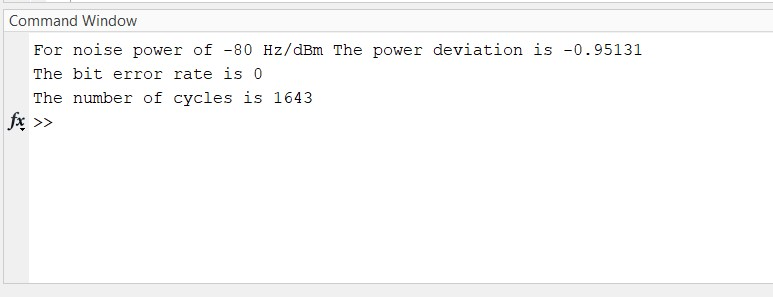
\includegraphics[scale=1]{Chapter 4/Figures/SISO System Performance}
\caption[SISO Tone Loading]{The performance of our SISO system. The number of cycles taken to transmit the bits is of particular importance to us.}
\label{fig:siso system performance}
\end{figure}

\begin{figure}[!htbp]
\centering
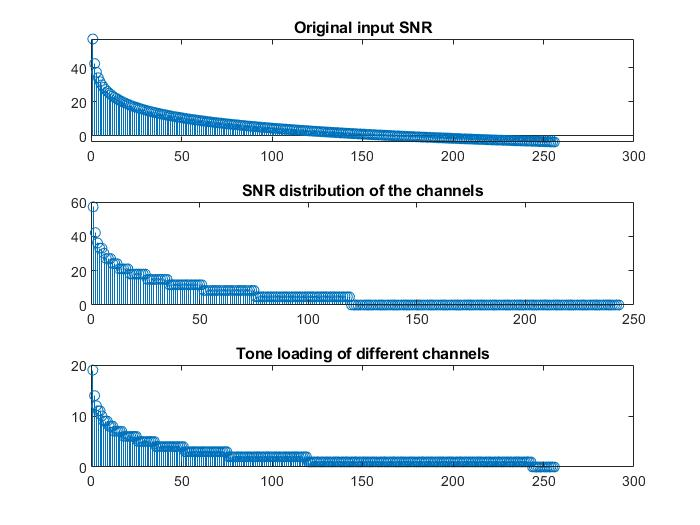
\includegraphics[scale=0.7]{Chapter 4/Figures/SISO Tone Loading}
\caption[SISO Tone Loading]{The tone loading profile of various subchannels for SISO mode.}
\label{fig:siso tone loading}
\end{figure}

\section{SIMO System Results}
The result for the \acrshort{simo} simulation is shown in figure \ref{fig:simo system performance}. The \acrshort{ber} is observed to be $0$, which is within the expected range. Also, the total power deviation due to rounding of the number of bits per tone is $-1.82$ dB which is less than our threshold value of $\pm 2$ dB.\\
We observe in figure \ref{fig:simo tone loading} that the subchannels with higher \acrshort{snr} have more bits loaded onto them which is the expected behavior of our tone loading algorithm.\\
To transmit $10^6$ bits, we need a total of $1051$ cycles of transmitting bits as per the tone loading profile in \ref{fig:simo tone loading}. This is done again in diversity mode. We shall see how using \acrshort{mimo} systems improve this rate.

\begin{figure}[!htbp]
\centering
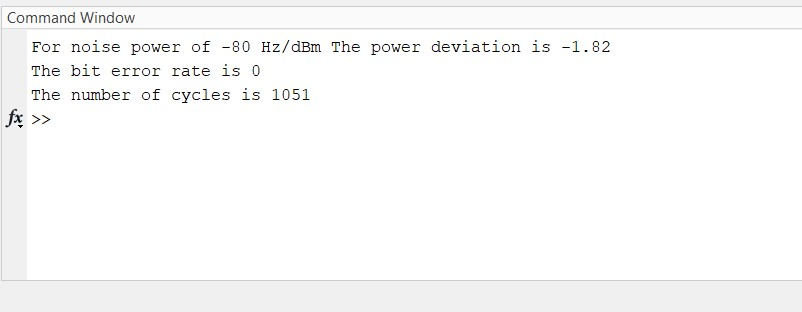
\includegraphics[scale=1]{Chapter 4/Figures/SIMO System Performance}
\caption[SIMO Tone Loading]{The performance of our SIMO system. The number of cycles taken to transmit the bits is of particular importance to us.}
\label{fig:simo system performance}
\end{figure}

\begin{figure}[!htbp]
\centering
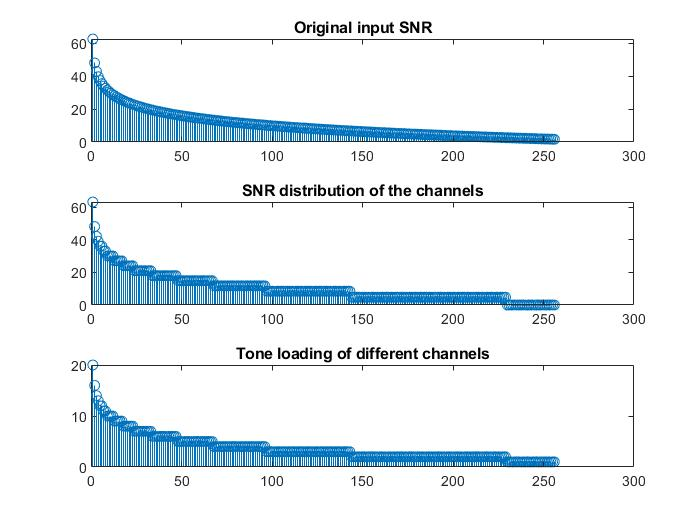
\includegraphics[scale=0.7]{Chapter 4/Figures/SIMO Tone Loading}
\caption[SIMO Tone Loading]{The tone loading profile of various subchannels for SIMO mode.}
\label{fig:simo tone loading}
\end{figure}

\section{MISO System Results}
The result for the \acrshort{miso} simulation is shown in the figure \ref{fig:miso system performance}. The \acrshort{ber} is observed to be $0$, which is within the expected range. We do not perform any tone loading as we use a Alamouti precoding scheme. It takes only $98$ cycles to transmit the $10^6$ bits.

\begin{figure}[!htbp]
\centering
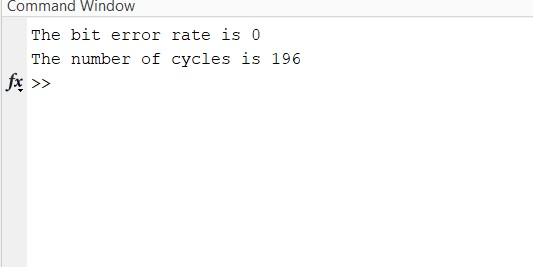
\includegraphics[scale=1]{Chapter 4/Figures/MISO System Performance}
\caption{MISO System Performance.}
\label{fig:miso system performance}
\end{figure}

\section{MIMO System Results}

\subsection{MIMO Diversity Case}
The result for the \acrshort{mimo} simulation in diversity case is shown in figure \ref{fig:mimo system performance diversity}. The \acrshort{ber} is observed to be $0$, which is within the expected range. Also, the total power deviation due to rounding of the number of bits per tone is $-1.3892$ dB which is less than our threshold value of $\pm 2$ dB.\\
We observe in figure \ref{fig:mimo tone loading diversity} that the subchannels with higher \acrshort{snr} have more bits loaded onto them which is the expected behavior of our tone loading algorithm.\\
Although we have many antenna paths to transmit $10^6$ bits, since we are operating in diversity mode we need a total of $1303$ cycles of transmitting bits as per the tone loading profile in \ref{fig:mimo tone loading diversity}. We shall see how operating \acrshort{mimo} in multiplexing mode can vastly improve this system performance.

\begin{figure}[!htbp]
\centering
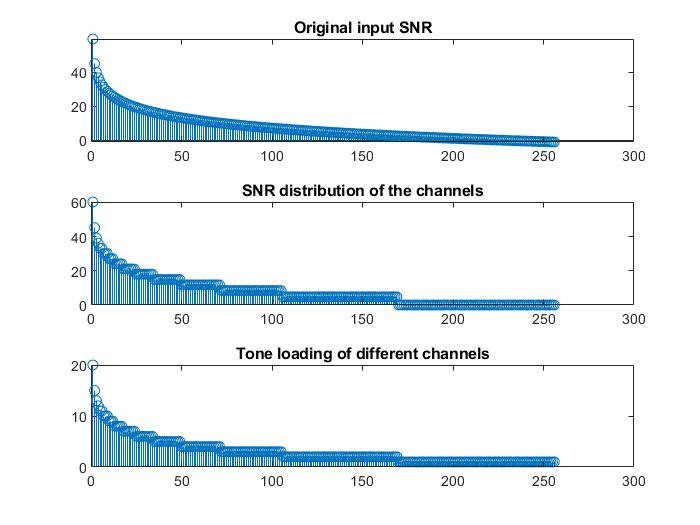
\includegraphics[scale=0.7]{Chapter 4/Figures/MIMO Tone Loading Diversity}
\caption[MIMO Tone Loading in Diversity Case]{The tone loading profile of various subchannels for MIMO in diversity mode.}
\label{fig:mimo tone loading diversity}
\end{figure}

\begin{figure}[!htbp]
\centering
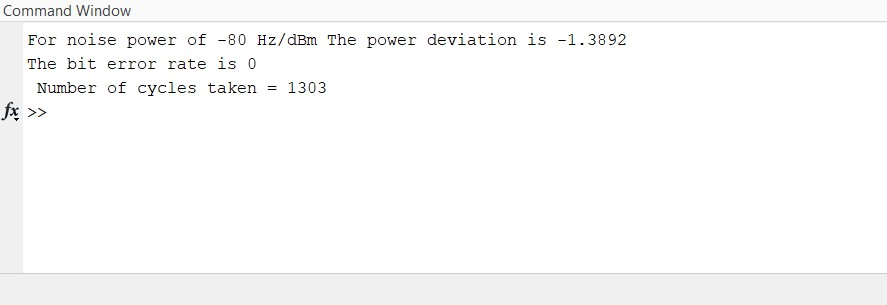
\includegraphics[scale=1]{Chapter 4/Figures/MIMO System Performance Diversity}
\caption[MIMO System Performance in Diversity Case]{The performance of our MIMO system. The number of cycles taken to transmit the bits is of particular importance to us.}
\label{fig:mimo system performance diversity}
\end{figure}

\subsection{MIMO Multiplexing Case}

The result for the \acrshort{mimo} simulation in multiplexing case is shown in figure \ref{fig:mimo system performance multiplexing}. The \acrshort{ber} is observed to be $0$, which is within the expected range. Also, the total power deviation due to rounding of the number of bits per tone is $-0.65038$ dB which is less than our threshold value of $\pm 2$ dB.\\
We observe in figure \ref{fig:mimo tone loading multiplexing} that the subchannels with higher \acrshort{snr} have more bits loaded onto them which is the expected behavior of our tone loading algorithm.\\
Since we have many antenna paths to transmit $10^6$ bits, we only $797$ cycles of transmitting bits as per the tone loading profile in \ref{fig:mimo tone loading diversity}. As we see, in the multiplexing case, the number of cycles have reduced considerably directly interfering higher data rates.

\begin{figure}[!htbp]
\centering
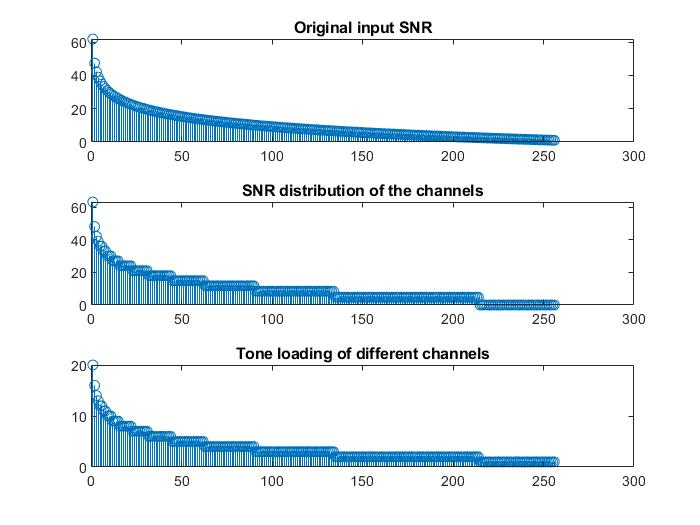
\includegraphics[scale=0.7]{Chapter 4/Figures/MIMO Tone Loading Multiplexing}
\caption[MIMO Tone Loading in Multiplexing Case]{The tone loading profile of various subchannels for MIMO in diversity mode.}
\label{fig:mimo tone loading multiplexing}
\end{figure}

\begin{figure}[!htbp]
\centering
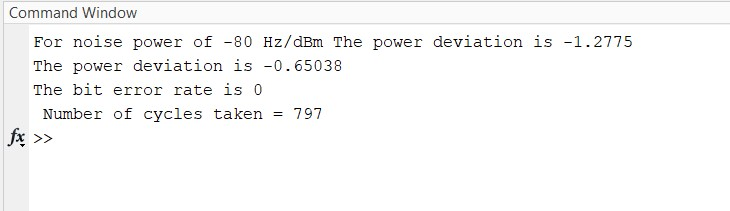
\includegraphics[scale=1]{Chapter 4/Figures/MIMO System Performance Multiplexing}
\caption[MIMO System Performance in Multiplexing Case]{The performance of our MIMO system. The number of cycles taken to transmit the bits is of particular importance to us.}
\label{fig:mimo system performance multiplexing}
\end{figure}

\subsection{MIMO Multiplexing with Inverse Channel Estimation Precoder}

The result for the \acrshort{mimo} simulation for multiplexing case with inverse channel estimation precoder is shown in the figure \ref{fig:mimo system performance inverse channel estimation}. The \acrshort{ber} is observed to be $0$, which is within the expected range. We do not perform any tone loading as we use a Inverse Channel Estimation precoding scheme. It takes only $98$ cycles to transmit the $10^6$ bits. We notice how by using suitable precoding the number of cycles reduce drastically.

\begin{figure}[!htbp]
\centering
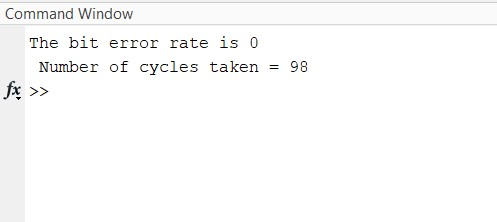
\includegraphics[scale=1]{Chapter 4/Figures/MIMO System Performance Inverse Channel Estimation}
\caption{MIMO System Performance with Inverse Channel Estimation Precoder.}
\label{fig:mimo system performance inverse channel estimation}
\end{figure}

\subsection{MIMO Multiplexing with Singular Value Decomposition Precoder}

The result for the \acrshort{mimo} simulation for multiplexing case with singular value decomposition precoder is shown in the figure \ref{fig:mimo system performance singular value decomposition}. The \acrshort{ber} is observed to be $0$, which is within the expected range. We do not perform any tone loading as we use a Singular Value Decomposition precoding scheme. It takes only $98$ cycles to transmit the $10^6$ bits. We notice how by using suitable precoding the number of cycles reduce drastically.

\begin{figure}[!htbp]
\centering
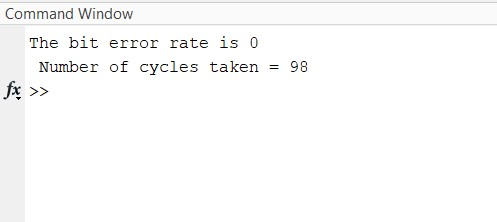
\includegraphics[scale=1]{Chapter 4/Figures/MIMO System Performance Inverse Channel Estimation}
\caption{MIMO System Performance with Singular Value Decomposition Precoder.}
\label{fig:mimo system performance singular value decomposition}
\end{figure}

\section*{Summary}
In this section we discussed the results of the simulations of our system in various configurations. We clearly see that data rates increase with multiplexing mode and also with precoding. Finally, in the last section we conclude our report and talk about the future scope of the report and how further improvements can be made to our system.






%Chapter 5 Result
\input{./Chapter 5/chapter 5 - Conclusion and Future Scope}

\backmatter
\clearpage
\printbibliography

\end{spacing}

\end{document}